\chapter{Data Set Generation}
\label{chp:dataset}
Due to the lack of labeled real-world data streams, stream mining algorithms are most of the time tested with synthesized data. Synthesized data has several advantages over poorly labeled real-world data streams. First of all, it is rather easy to produce. It has significantly less storage overhead. It is easier to control synthesizing parameters to generate data sets with the desired concept drift, recurrence, etc. scenarios.

In this chapter, we briefly discuss some of such generators. For our experimentations we used random radial basis function (RBF) generator. Thus, we  discuss the generation process and the generated stream's properties from a random RBF generator in greater details. We then describe the modifications in the generation process to introduce variable speed RBF streams.

\section{Existing Stream Generators}
A number of generators have been introduced in literature in the past decades: SEA concept generator, STAGGER concepts generator, rotating hyperplane generator, random RBF generator, waveform generator are some of the commonly used ones. 

\subsection*{SEA Concepts Generator}
The SEA concept generator is introduced in~\cite{street01:sea} to generate a synthetic data set with abrupt concept drift. It uses three parameters valued between $0$ and $10$ inclusive. The points of the data set are divided into blocks of different concepts. Classification within the each block is controlled using the input parameters along with a threshold value.

\subsection*{STAGGER Concepts Generator}
STAGGER is one of the early methods developed for stream generation by Schlimmer et al.~\cite{schlimmer86:stagger}. Binary concepts are generated from three attributes. Attributes are size, shape, and color. Each of the attributes has three possible values. Small, medium, and large are the sizes; circle, triangle, and rectangle are the shapes; and red, blue, and green are the colors. $27$ combinations are being mapped into a binary class by this generator.

\subsection*{Rotating Hyperplane Generator}
A rotating hyperplane generator is introduced in the evaluation of CVFDT~\cite{hulten01:cvfdt}. Hyperplanes can effectively be used to simulate concept drifting environments. A hyperplane in a $d$-dimensional space is a set of points $x$ that satisfies following equation:
\[
    \sum_{i=1}^{d} w_i x_i = w_0 = \sum_{i=1}^{d} w_i
\]
where $x_i$ is the $i$th coordinate of $x$. The hyperplane works as the boundary between two of the binary classes. By controlling the orientation and position of the hyperplane concept drift can be controlled. 

\subsection*{Wavefront Generator}
The wavefront generator is a data set available at the UCI machine learning repository~\cite{internet:ucirepo}. Two or three base waves are used to generate a data set of three different classes of waveforms. The prediction task is to predict the classes of waveforms. The optimal Bayes classification rate is known to be $86\%$. There are two variations of this generator. Wave21 uses 21 numeric noisy attributes, and wave40 uses 19 more irrelevant attributes along with original 21.

\subsection*{LED Generator}
LED generator is also available at the UCI machine learning repository~\cite{internet:ucirepo}. The prediction task for this data set is to predict the digit displayed on a seven segment LED display. Each segment has $10\%$ chance of being inverted. The optimal classification using na\"ive Bayes on this data set is  $74\%$. 

\subsection*{Random Radial Basis Function Generator}
All the generators mentioned above are relatively simple and easy to use. However, it is harder to model a complex scenario with those generators. Hypothesis spaces for these generators are not very large, except for the rotating hyperplane generator. But with the rotating hyperplane generator it is harder to produce overlapping space and outliers. A random radial basis function (RBF) generator is therefore introduced to generate a complex concept type that is not straight forward to approximate, especially with a decision tree model.

RBF generator starts by selecting a fixed number of random centroids, each at a random position in the hyperspace with a standard deviation, class label and weight. Instances are generated by selecting a centroid at random and generating a random point near that centroid by maintaining a Gaussian distribution with the previously selected standard deviation and the location of the centroid as mean. Direction of the deviation is selected at random. The class label of the instance is assigned to be the one of the selected centroid. The selection of centroid depends on the weights of the centroids, so that centroids with higher weights get higher chances to get selected.
\begin{figure}[htbp] 
    \begin{center}
        \begin{tabular}{cc}
            \hspace{-5mm}\resizebox{90mm}{!}{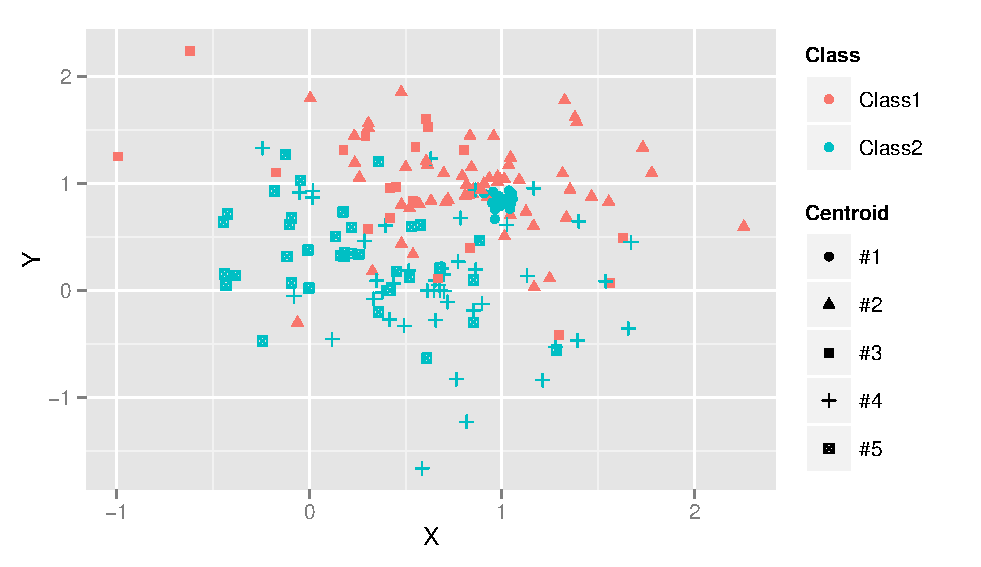
\includegraphics{figs/rbf5x2.pdf}} &
            \hspace{-10mm}
            \resizebox{70mm}{!}{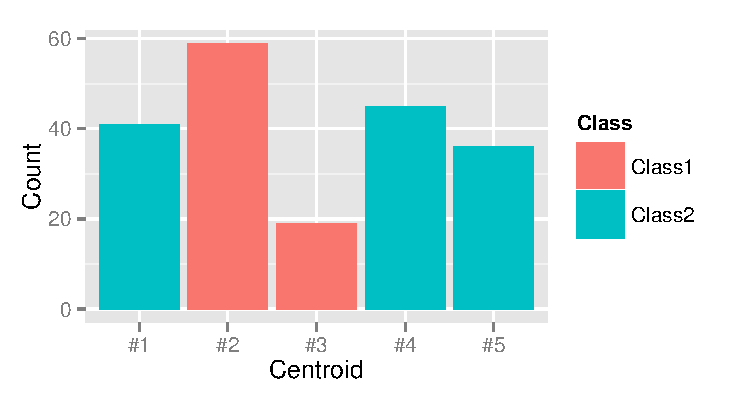
\includegraphics{figs/rbf5x2-hist.pdf}} \\
            \scriptsize{(a)\vspace{2mm}} &
            \scriptsize{(b)}    
        \end{tabular}
        \caption{RBF data generation in 2D space (a) distribution (b) histogram}
        \label{fig:ds:rbf}
    \end{center}
\end{figure}

Figure~\ref{fig:ds:rbf} illustrates a generated data set on two dimensional space with no concept drift. Figure~\ref{fig:ds:rbf}a shows the distribution of the instances, and Figure~\ref{fig:ds:rbf}b presents the histogram of 5 centroids from which data are generated. The differences among the centroids' weights are clearly visible here. However, it is to notice here is that the overall data set is somewhat balanced in terms of class distribution.

\begin{figure}[htbp] 
    \begin{center}
        \begin{tabular}{cc}
            \resizebox{75mm}{!}{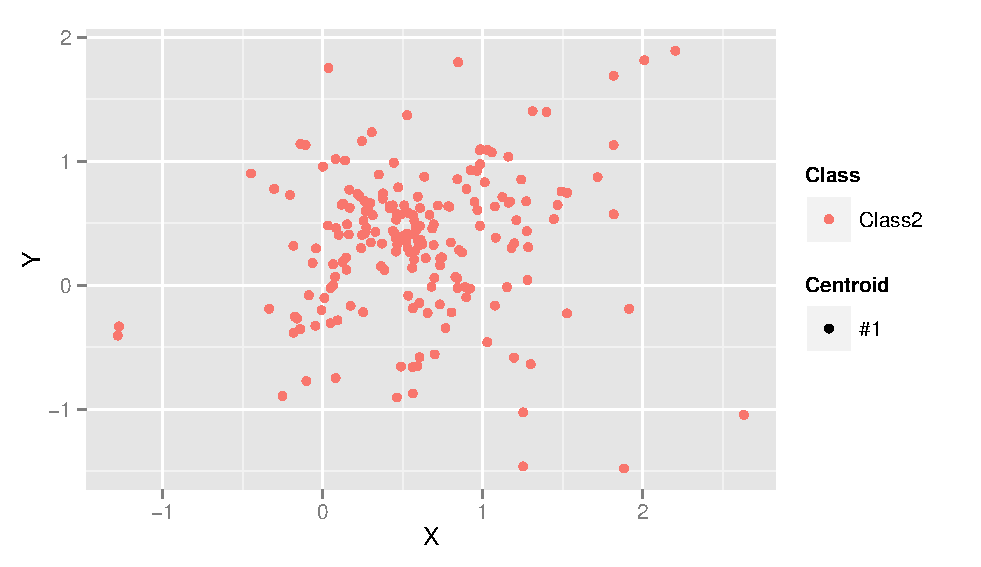
\includegraphics{figs/drift-0.pdf}} &
            \resizebox{75mm}{!}{\includegraphics{figs/{drift-0.01}.pdf}} \\
            \scriptsize{(a)} & \scriptsize{(b)\vspace{2mm}} \\
            \resizebox{75mm}{!}{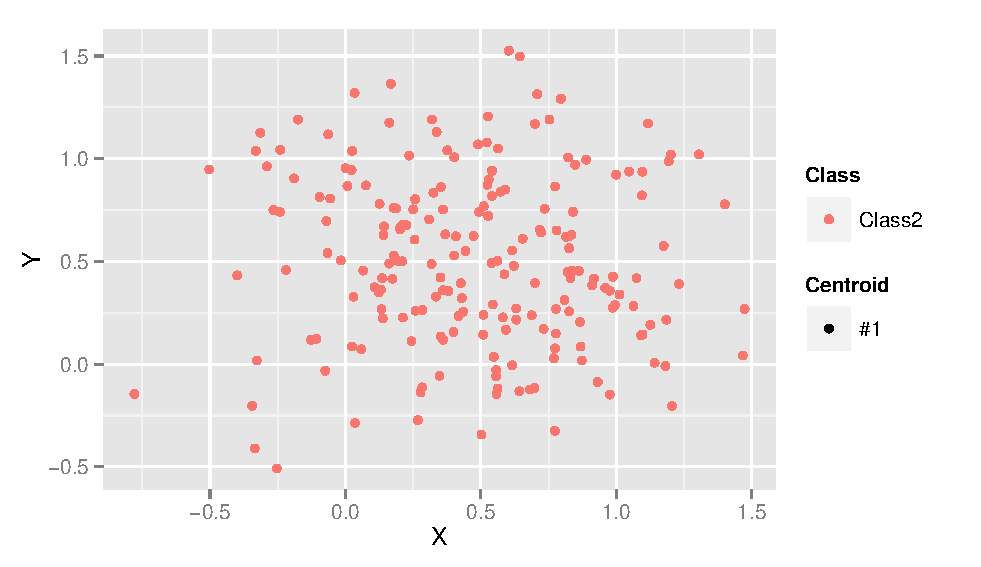
\includegraphics{figs/drift-1.pdf}} &
            \resizebox{75mm}{!}{\includegraphics{figs/{drift-0.1}.pdf}} \\
            \scriptsize{(c)} & \scriptsize{(d)}
        \end{tabular}
        \caption{RBF data generation with concept drift. Drift coefficient: (a) 0, (b) 0.01, (c) 0.1, and (d) 1}
        \label{fig:ds:rbfdrift}
    \end{center}
\end{figure}
Next, in Figure~\ref{fig:ds:rbfdrift} we present 4 generated data sets with only one centroid, hence all instance belongs to one class. Figure~\ref{fig:ds:rbfdrift}a, \ref{fig:ds:rbfdrift}b, \ref{fig:ds:rbfdrift}c, and \ref{fig:ds:rbfdrift}d have a drift coefficient of 0, 0.01, 0.1, and 1 respectively. As it can be seen, the instances are more compact when there is no concept drift. The introduction of a small concept drift gradually moves the concepts away. With a higher drift coefficient, instances become sparser.

We retain most of these properties of a RBF generator in creating our Variable Speed RBF Stream. We manipulate the generation process to achieve our desired properties in the data set. We want the data set to be balanced in terms of the binary class distribution. We also want some centroids to produce more data, possibly with higher drift while some centroids with very little drift produce fewer data in a certain time frame. With these goals, we present the data generation process for variable speed RBF Stream in the next chapter.

\section{A New Approach to Generate Variable Speed RBF Streams}
To generate a variable speed RBF stream, we replace the concept of centroids with pools of centroids. At the start of the generation process a sufficient number of centroids is generated and assigned randomly to a user specified number of pools. The generation process of centroids remain exactly the same as the RBF generator: a randomly chosen point in the hyper-space with a randomly assigned class label. Instances generating from each centroid have this point as the mean of the normal distribution with a randomly selected standard deviation. After assigning these centroids into pools, the pools are assigned relative weights. We have used linearly increasing and quadratically increasing weights for experiments. Drift coefficients associated with all the centroids within a pool are the same and also follow  a quadratic rate among the pools. As we mentioned before, slower pools i.e. pools with lower weights have lower drift coefficients than the pools with higher weights.

\begin{algorithm}[htbp]
    \caption{Variable Speed RBF Generator}
    \label{alg:vsrbf}
    \DontPrintSemicolon
    \SetKwInOut{Input}{Input} \SetKwInOut{Output}{Output} 
    
    \Input{$c$: Number of classes \\
        $d$: Number of attributes \\
        $p$: Number of pools \\
        $b$: Number of batch size \\
        $n$: Size of the stream
    } 
    \Output{$D$: A data stream}
    
    \Begin{
        Create $P$ pools \\
        Generate $m$ centroids		  	\tcp*[f]{Sufficiently high number, $n>>p$} \\
        Distribute $m$ centroids to $p$ pools randomly \\
        Let $w_i$ is the weight of $i$th pool \\
        $w_i = a * i^2$		  			\tcp*[f]{Associate each pool with a quadratic weight} \\
        Let $a_i$ is the activation percentage of $i$th pool \\
        
        \While{n > 0} {
            \ForEach{$P_i \in pools$} {
                Randomly select $a_i$ fraction of centroids in $P_i$ \\
            }
            
            \ForEach{$P_i \in pools$} {
                $n_i = w_i * b / w$ where $w = \sum w_i$ \\
                Generate $n_i$ instances \\
            }
            Randomly shuffle all generated instances \\
            Add instances to $D$ \\
            $n = n - b$ \\
        }
        Return $D$
    }
\end{algorithm}

To mimic concept evolution and recurrence, we associate each pool with an activation percentage. The activation percentage determines the percentage of centroids within the pool that are activated. If a centroid is not activated, it will not produce any instance until it gets activated again. Slower pools has higher activation percentages. With these settings, the pool with the highest weight will produce a burst of instances belonging to only a few centroids while the pool with the lowest weight will produce small number of instances from a higher number of centroids. As mentioned before, these centroids are also associated with less drift. Thus, essentially we would get slow but consistent concepts.


\begin{figure}[htbp] 
    \begin{center}
        \begin{tabular}{cc}
            \hspace{-5mm}\resizebox{90mm}{!}{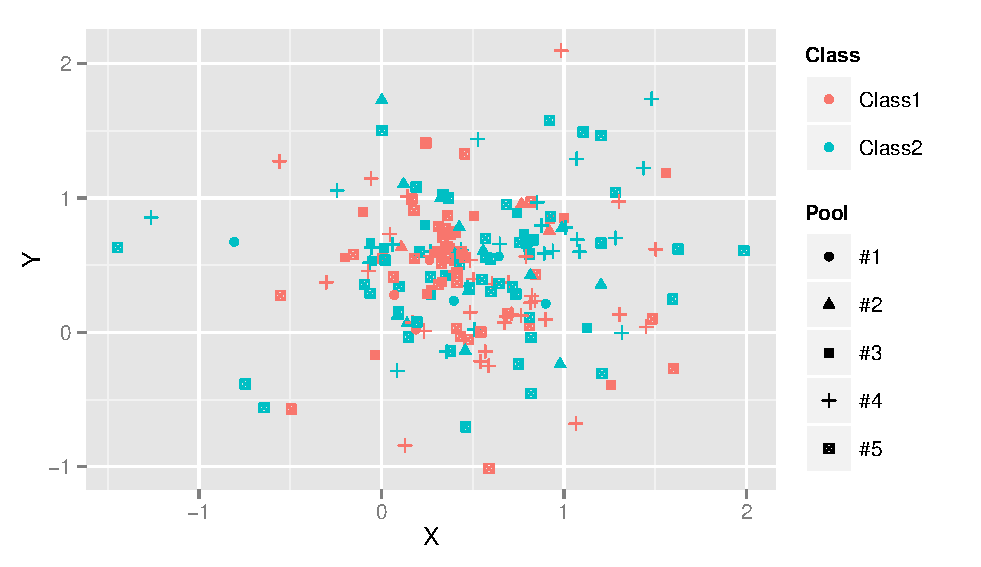
\includegraphics{figs/var5x2.pdf}} &
            \hspace{-10mm}
            \resizebox{70mm}{!}{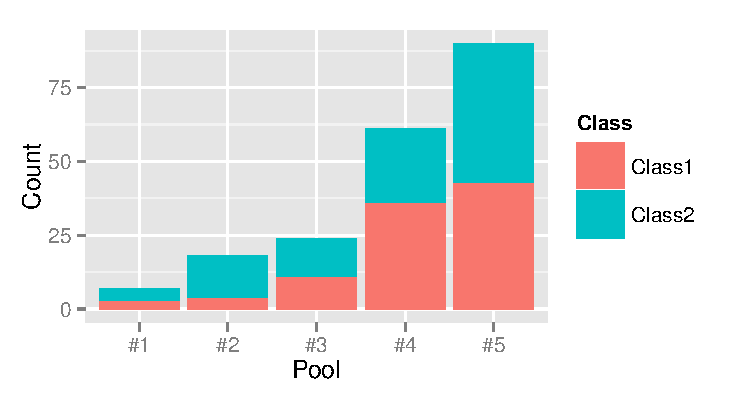
\includegraphics{figs/var5x2-hist.pdf}} \\
            \scriptsize{(a)\vspace{2mm}} &
            \scriptsize{(b)}    
        \end{tabular}
        \caption{Variable speed data generation in 2D space (a) distribution (b) histogram}
        \label{fig:ds:varspd}
    \end{center}
\end{figure}

For the ease of implementation, we achieved this weight  variation and activation among the pools by generating instances in batches. Each batch starts by configuring the pools. The activation of centroids is changed randomly based on the activation percentage at each configuration. It randomly activates the required number of centroids based on the associated activation percentage of the pools. For each batch, each pool generates a certain number of instances depending on its weight. Contributions from all the pools are then shuffled randomly. The batches serve as reservoirs. Once a reservoir gets depleted, the next batch fills the reservoir. Algorithm~\ref{alg:vsrbf} presents pseudo-code of the generation process.

Figure~\ref{fig:ds:varspd} presents a generated data set with 5 pools. As the histogram indicates, the $4^{th}$, and $5^{th}$ pools produce significantly higher number of instances compared to the $1^{st}$, $2^{nd}$, or $3^{rd}$ pool. However, close inspection at Figure~\ref{fig:ds:varspd}a would reveal that instances from these pools are more compact than the other two pools with a higher instance count. Another important property to notice here is that even though there is significant difference in the number of instances produced from each pool, the overall data set is somewhat balanced.

\begin{figure}[htbp] 
    \begin{center}
        \begin{tabular}{c}
            \resizebox{130mm}{!}{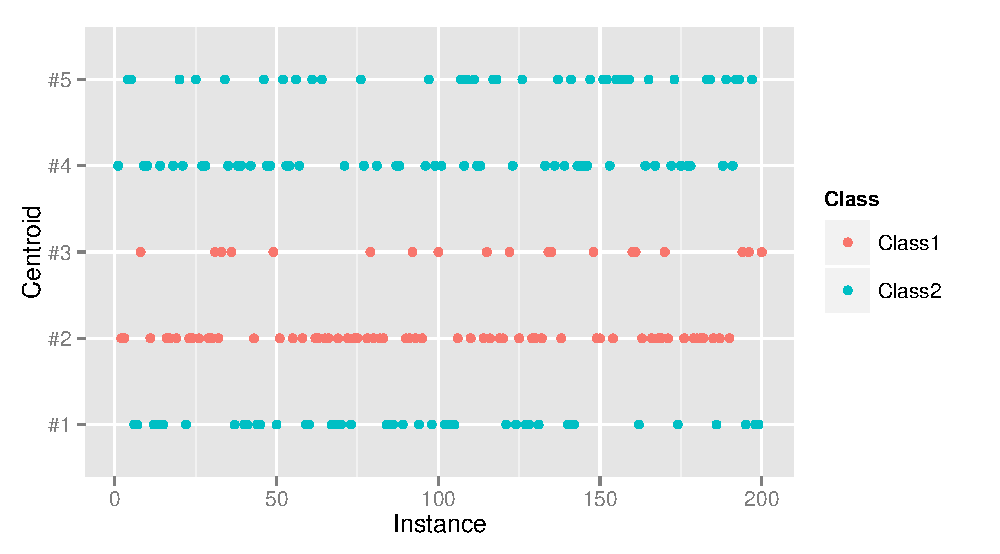
\includegraphics{figs/rbf-ivc.pdf}} \\
            \scriptsize{(a)\vspace{2mm}} \\
            \resizebox{130mm}{!}{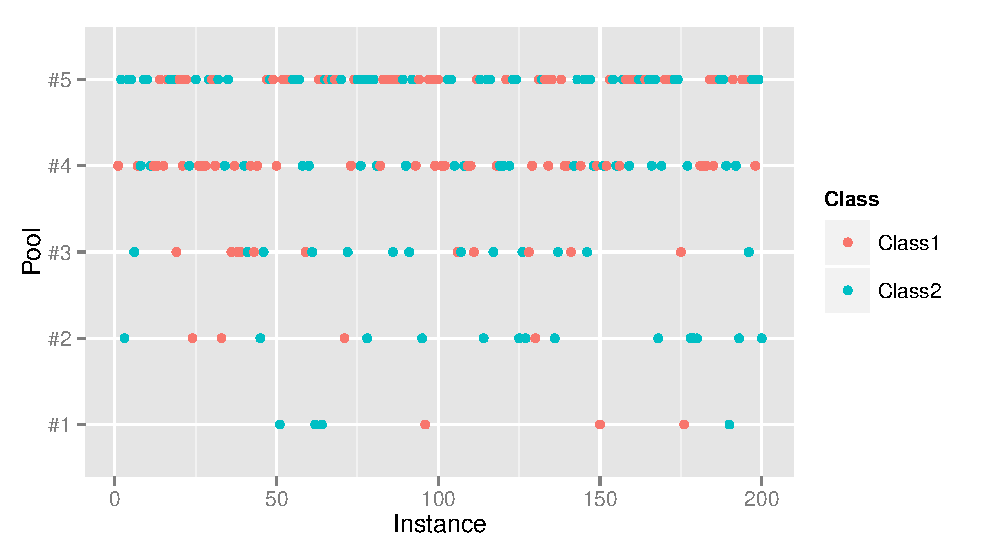
\includegraphics{figs/var-ivp.pdf}} \\
            \scriptsize{(b)}    
        \end{tabular}
        \caption{Timeline of instances (a) random RBF generator (b) variable-speed RBF generator}
        \label{fig:ds:ivcp}
    \end{center}
\end{figure}

Lastly, it is to be noticed here that even though slower pools produce less instances than the faster ones, they are expected to be distributed in the entire time frame. Figure~\ref{fig:ds:ivcp} confirms that expectation. In Figure~\ref{fig:ds:ivcp}a, it shows a timeline for a generated data set with the RBF generator. It shows that each centroid generates throughout the generation process. Similarly, in the data set generated by the variable speed RBF generator data are generated by every pool, throughout the generation process (Figure~\ref{fig:ds:ivcp}b). The slowest pool produces less data, but it does not do so in a fraction of the time frame. Moreover, in Figure~\ref{fig:ds:ivsc}, it shows a timeline for the contributing centroids. Values are set such that at each timestamp there are about 75 instances, thus there are 3 different timestamps in the plot. Looking into the figure, it can be easily seen that for the 5th pool, at the beginning only Centroid10 is producing data. For the rest of the two timestamps Centroid30 is producing data. Similarly, for the 4th pool, at the beginning two centroids produces data: Centroid01 produces Class2 data and Centroid24 produces data from Class1. They also stop producing for the next two timestamps. For Pool3, Centroid29 is active all the time, while other change their activation. For another two pools most of the centroids are mostly active for all three timestamps.


\begin{figure}[htbp] 
    \begin{center}
        \resizebox{130mm}{!}{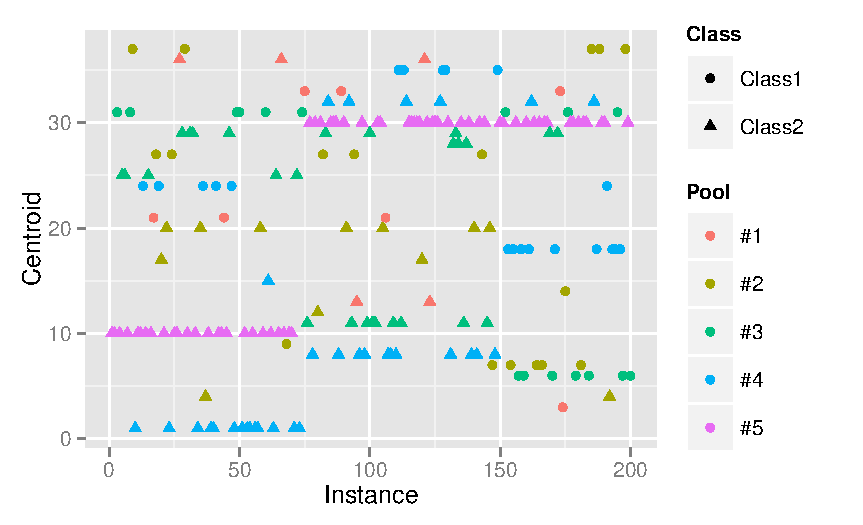
\includegraphics{figs/var-ivsc.pdf}}
        \caption{Timeline for contributing centroid in variable-speed RBF generator}
        \label{fig:ds:ivsc}
    \end{center}
\end{figure}



The discussions so far in this chapter, demonstrate that the variable speed RBF generator is able to produce a stream that mimics the behaviors or properties of the streams introduced in Section~\ref{sec:intro:motiv}, which is the basic motivation for our algorithm. In the next chapter, we evaluate the algorithms with these data generation schemes.
